\documentclass{article}

\usepackage{shyne}

% document format
\topmargin 0in
\oddsidemargin 0in
\evensidemargin 0in
\headheight 0in
\headsep 0in
\topskip 0in
\textheight 9in
\textwidth 6.5in
\linespread{1.3}

\begin{document}

\begin{flushleft}
\section*{Group Work - Chapter 10}
\paragraph{1} The file ``Galton-mother-daughter.csv" contains a subset 50 subjects from Galton's mother/daughter height data.
\begin{enumalpha}
\item Create a scatterplot of the data. Does there appear to be a linear relationship between mother's heights and daughter's heights?\\
\medskip
\bt{There does appear to be a linear relationship.}\\
\medskip
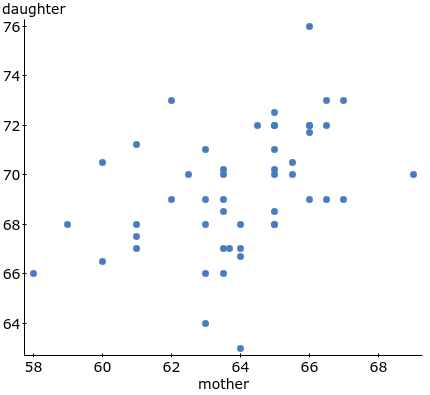
\includegraphics[width=4in]{images/grp10_Q1_a}
\vspace{.5in}
\item Conduct a correlation hypothesis test at $\alpha = 0.05$ significance level. If there is significant correlation, how would you describe the strength of the correlation?\\
\medskip
$\bv{r = 0.427, \, p = 0.002 < \alpha = 0.05}$. \bt{Reject $\bv{H_0}$. \\ 
There is evidence that heights of mothers and daughters are correlated.\\
Mother and daughter heights are moderately correlated.}
\newpage
\item Find the estimated regression line for the relationship between mother's heights (predictor variable) and daughter's heights (response variable)? Is the slope significantly different than zero?\\
\medskip
\bt{daughter = 38.235 + 0.487 mother}\\
$\bv{t = 3.2742973, \, p = 0.002}$. \bt{The slope is significantly different than zero.}
\vspace{.5in}
\item What is the best predicted daughter's height for a mother that is 56 inches tall? Is it appropriate to make such a prediction?\\
\medskip
\bt{Since we have a significant correlation, use the regression equation for the prediction.}\\
\bt{daughter = 38.235 + 0.487 (56) = 65.507}\\
\bt{Or, from StatCrunch, daughter = 65.51055}\\
\medskip
\bt{Mothers' heights range from 58 to 69 inches. Thus, making a prediction for a mother's height of 56 inches is not appropriate.}


\end{enumalpha}



\newpage
\paragraph{2} The Prime Minister of Freedonia wishes to improve the economic strength of his country. He instructs his finance minister to study the relationship between tacos consumed and Freedonia's GDP. The results by month for last year are in the file ``Freedonia.csv" on D2L. The data represents tacos consumed per capita and GDP in billlions of Freedonia's national currency (Fr\$).
\begin{enumalpha}
\item Create a scatterplot of the data. Does there appear to be a linear relationship between tacos consumed and Freedonia's GDP?\\
\medskip
\bt{There does appear to be a linear relationship, with a couple of outliers.}\\
\medskip
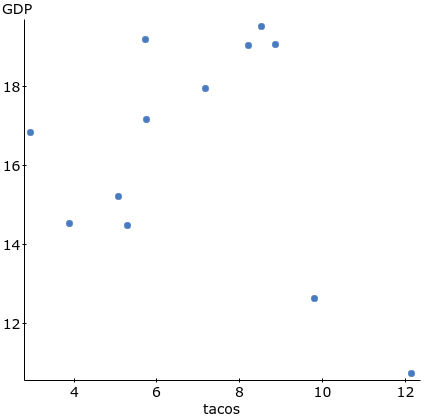
\includegraphics[width=4in]{images/grp10_Q2_a}
\vspace{.5in}
\item Conduct a correlation hypothesis test at $\alpha = 0.05$ significance level. If there is significant correlation, how would you describe the strength of the correlation? Would it be worthwhile to also test the correlation with GDP measured in US dollars?\\
\medskip
$\bv{r = -0.256, \, p = 0.4226 > \alpha = 0.05}$. \bt{Fail to reject $\bv{H_0}$. \\ 
There is not evidence that taco consumption and Freedonia GDP are correlated.\\
Units don't affect correlation values, so it is not useful to also test with GDP measures in US dollars.}
\newpage
\item Find the estimated regression line for the relationship between tacos consumed (predictor variable) and GDP (response variable)? Is the slope significantly different than zero?\\
\medskip
\bt{GDP = 18.281385 - 0.27577839 tacos}\\
$\bv{t = -0.83608443, \, p = 0.4226}$. \bt{The slope is not significantly different than zero.}
\vspace{.5in}
\item What is the best predicted GDP for a month in which 9.5 tacos are consumed per capita? Is it appropriate to make such a prediction?\\
\medskip
\bt{Since we do not have a significant correlation, use the mean GDP as the predictor.}\\
\bt{Mean GDP = 16.367}\\
\medskip
\bt{Tace consumption ranges from 2.939 to 12.125 tacos per capita. Thus, making a prediction for taco consumption of 9.5 is appropriate. However, since the correlation is not significant, the prediction would be the same regardless.}
\end{enumalpha}

\newpage
\paragraph{3} The file ``MCA\_scores\_17.csv" on D2L contains average math MCA scores for 11th graders in 2017 by MN public school district, as well as percentage of 11th graders receiving free lunches in the district. Districts with missing data and charter schools are excluded.
\begin{enumalpha}
\item Create a scatterplot of the data. Does there appear to be a linear relationship between percentage of students receiving free lunch and average MCA scores?\\
\medskip
\bt{There does appear to be a linear relationship.}\\
\medskip
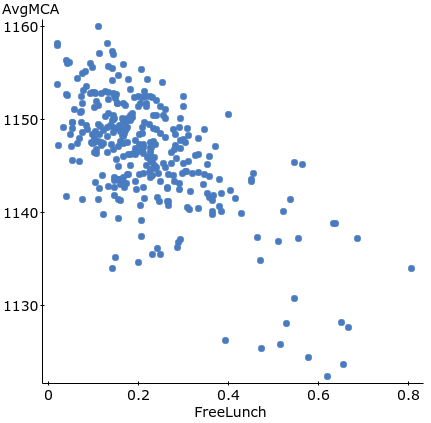
\includegraphics[width=4in]{images/grp10_Q3_a}
\vspace{.5in}
\item Conduct a correlation hypothesis test at $\alpha = 0.01$ significance level. If there is significant correlation, how would you describe the strength of the correlation?\\
\medskip
$\bv{r = -0.652, \, p <0.0001 < \alpha = 0.01}$. \bt{Reject $\bv{H_0}$. \\ 
There is evidence that proportion of free lunch students in a district and average MCA scores are correlated.\\
Proportion of free lunch students in a district and average MCA scores are moderately correlated, close to highly correlated.}
\newpage
\item Find the estimated regression line for the relationship between percentage of students receiving free lunch (predictor variable) and average MCA scores (response variable)? Is the slope significantly different than zero?\\
\medskip
\bt{AvgMCA = 1153.070 - 30.173 FreeLunch}\\
$\bv{t = -15.403601, \, p < 0.0001}$. \bt{The slope is significantly different than zero.}
\vspace{.5in}
\item What is the best predicted average MCA score for a district that has 45\% of 11th grade students receiving free lunch? Is it appropriate to make such a prediction?\\
\medskip
\bt{Since we have a significant correlation, use the regression equation for the prediction.}\\
\bt{AvgMCA = 1153.070 - 30.173 (0.45) = 1139.492}\\
\bt{Or, from StatCrunch, AvgMCA = 1139.4923}\\
\medskip
\bt{Proportions of free lunch students range from 0.0202 to 0.8046. Thus, making a prediction for a free lunch proportion of 0.45 is appropriate.}
\end{enumalpha}



\end{flushleft}
\end{document}